	\chapter{Das Strahlungstransportproblem}
	\label{sec:radiative_transfer}
	
	Das Verhalten von Licht l"asst sich (nach heutigem wissenschaftlichen Stand) durch die {\em Quantenelektrodynamik}\footnote{siehe z.B. \citet{Feynman:1990p11684}} in allen Details vollst"andig beschreiben. Es beinhaltet solche Ph"anomene wie Dispersion, Brechung, Interferenz, Photon--Photon--Interaktion, etc. Diese Effekte sind h"aufig dann am bedeutendsten, wenn die Ausma"se der betrachteten Objekte von der Gr"o"senordnung der Wellenl"ange des Lichtes sind. Auf der anderen Seite beschreibt die {\em geometrische Optik} die rein makroskopische lineare Ausbreitung gro"ser Mengen von Photonen ohne obengenannte Wellen--Ph"anomene zu ber"ucksichtigen.
	
	Beim Strahlungstransportproblem (STP) sind wir an einer {\em ph"anomenologischen} Beschreibung interessiert. Das heisst wir wollen die Effekte des Lichtes modellieren, die in typischen Anwendungen durch optische Instrumente (Auge, Teleskope mit Photoplatten/CCD--Chips) gemessen werden k"onnen. Dies bedeutet, das wir haupts"achlich eine geometrische Beschreibung des Lichtes in Form eines Teilchentransportproblems ansetzen aber relevante quantenmechanische Effekte wie Photonen--Streuung in erster Ordnung lokal mitber"ucksichtigen (z.B. in Form einer Streuphasenfunktion).
	
	Die folgende Darstellung und Herleitung orientiert sich an \citep{Arvo:1993p9035}
	
	\section{Das Strahlungstransportproblem als Teilchentransportproblem}
	Um Strahlungstransport als Teilchentransportproblem behandeln zu k"onnen m"ussen folgende Bedingungen erf"ullt sein
	\begin{itemize}
		\item{Die Teilchen m"ussen so klein und zahlreich sein, das ihre statistische Verteilung als kontinuierlich angesehen werden kann}
		\item{Zu jedem Zeitpunkt l"asst sich ein Teilchen komplett durch seinen Positionsvektor, Geschwindigkeitsvektor und eventuelle interne Zust"ande (wie Polarisation, Frequenz, Ladung, Spin, etc.) charakterisieren}
	\end{itemize}
	Diese Annahmen sind f"ur Photonen und die uns interessierenden r"aumlichen Entfernungen erf"ullt.
	Dar"uber hinausgehend machen wir im Rahmen dieser Arbeit folgende Annahmen:
	\begin{itemize}
		\item{Die Materialeigenschaften "andern sich bei Variation des Ortes in der Gr"o"senordnung der Wellenl"ange nur wenig}
		\item{Das Strahlungsintensit"atsfeld ist station"ar (d.h. innerhalb der typischen Zeiten, die ein Photon braucht um das Simulationsgebiet zu durchqueren, k"onnen die Materialeigenschaften als statisch angenommen werden)}
		\item{Photonen werden ausschliesslich elastisch gestreut}
		\item{der Raum wird als euklidisch angenommen (d.h. es werden keine relativistischen Effekte ber"ucksichtigt)}
	\end{itemize}
	Die Annahme ausschliesslich elastischer Streuvorg"ange erlaubt es uns, dass Strahlungstransportproblem f"ur jede Wellenl"ange getrennt zu betrachten, da Photonen bei elastischer Streuung ihre Wellenl"ange nicht "andern und somit den Strahlungstransport in anderen Wellenl"angen nicht beeinflussen. Daher behandeln wir im Folgenden nur das monochromatische Strahlungstransportproblem, in dem Wissen, da"s der polychromatische Fall immer als eine Reihe von monochromatischen Problemen behandelt werden kann. Aufgrund der monochromatischen (und damit monoenergetischen) Annahme ist der Teilchenimpuls und somit die Teilchengeschwindigkeit konstant. Daher reicht es zur vollst"andigen Beschreibung eines Teilchenzustandes aus, wenn wir nur die Position $\location{r}$ (entsprechend drei Freiheitsgraden) und die Bewegungsrichtung $\omega$ (entsprechend zwei Freiheitsgraden) des Teilchens angeben. Wir k"onnen nun ein Teilchen als Punkt des zugeh"origen f"unf--dimensionalen Phasenraums $\mathbb{R}^3 \times \mathcal{S}^2$ identifizieren, wobei $\mathbb{R}^3$ den euklidischen Raum und $\mathcal{S}^2$ die Einheitskugel im $\mathbb{R}^3$ meint.
	
	Um die statistische Verteilung unserer Teilchen im Phasenraum zu jedem Zeitpunkt spezifizieren zu k"onnen f"uhren wir die Phasenraumdichte $n$ ein, soda"s $$n(\location{r},\omega,t)\,d\location{r}\,d\omega$$ der Anzahl Teilchen entspricht, die sich zum Zeitpunkt $t$ in einem infinitesimalen Volumen $d\location{r}$ um $\location{r} \in \mathbb{R}^3$ befinden und sich in eine Richtung bewegen, die innerhalb eines infinitesimalen Raumwinkels $d\omega$ um $\omega \in \mathcal{S}^2$ liegt. Damit hat $n$ die Einheit $\text{m}^{-3}\text{sr}^{-1}$. Die Phasenraumdichte trifft keine Aussage "uber Materialeigenschaften oder innere Zust"ande der Teilchen, wie Masse oder Frequenz, sondern beschreibt lediglich deren Anzahldichte im Phasenraum. Physikalisch relevante Gr"osen (wie z.B. die Intensit"at) f"uhren wir sp"ater (in Abschnitt \ref{subsec:strahlungsgroessen}) auf die Phasenraumdichte zur"uck. An dieser Stelle erlaubt die abstraktere Natur von $n$ aber eine klarere Darstellung der wesentlichen Verhaltensweisen der Teilchen. Von der Phasenraumdichte lassen sich alle f"ur uns interessanten Gr"osen prinzipiell ableiten, f"ur die folgende Herleitung ist es aber praktischer wenn wir uns die Rate der Teilchen, die eine imagin"are Fl"ache durchqueren, anschauen.
	
	Sei $d\location{A}$ eine infinitesimales Fl"achenelement, $\omega$ die Fl"achennormale von $d\location{A}$ und $d\omega$ ein infinitesimales Raumwinkelelement, das $\omega$ beinhaltet (siehe Abb.~(\ref{fig:phasespacefluxsurface})). Betrachten wir nun die Teilchen, welche die Fl"ache $d\location{A}$ in einem Zeitraum $dt$ mit Bewegungsrichtung innerhalb $d\omega$ passieren. Alle diese Teilchen liegen im Volumen $d\location{A}\,ds$ wobei $ds=v\,dt$ und $v$ die Geschwindigkeit der Teilchen ist. Nehmen wir an, da"s $\location{r}$ innerhalb diese Volumens liegt, ist die Anzahl der Teilchen $$n(\location{r},\omega,t)\,d\location{A}\,ds\,d\omega.$$ Wenn wir stattdessen aber nach der Rate fragen, mit der die Teilchen $d\location{A}$ passieren, erhalten wir den Phasenraumflu"s $$\phi(\location{r},\omega,t):=v\,n(\location{r},\omega,t)$$ mit der Einheit $[\phi]=\text{m}^{-2}\text{sr}^{-1}s^{-1}$. Die Teilchenanzahl in $d\location{A}\,ds$ mit dem Phasenraumflu"s ausgedr"uckt ist $$\phi(\location{r},\omega,t)\,d\location{A}\,d\omega\,dt.$$
	\begin{figure}
		\centering
		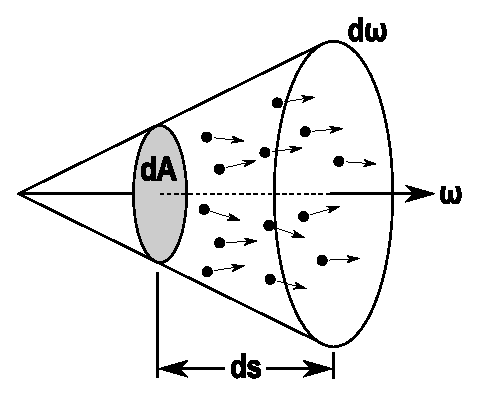
\includegraphics[height=0.3\textheight]{phasespacefluxsurface.eps}
		\caption{Teilchen, die das infinitesimale Fl"achenelement $d\location{A}$ durchqueren und sich in eine Richtung innerhalb des infinitesimalen Raumwinkelelements $d\omega$ um die Fl"achennormale $\omega$ von $d\location{A}$ bewegen.}
		\label{fig:phasespacefluxsurface}
	\end{figure}
	Der Phasenraumflu"s ist ebenso wie die Phasenraumdichte eine fundamentale Gr"ose aus der wir alle anderen interessanten Gr"osen ableiten k"onnen. Im Folgenden werden wir uns aber meist auf den Phasenraumflu"s beziehen.
		
	Unser Ziel ist es nun eine Bilanzgleichung f"ur die Teilchen in einem beliebigen Teil $V \times \Omega$ des Phasenraums (siehe Abb.~(\ref{fig:phasespacevolume})) aufzustellen. Dabei ist $V \subset \mathbb{R}^3$ ein Teilvolumen des $\mathbb{R}^3$ und $\Omega \subset \mathcal{S}^2$ ein beliebiger Raumwinkel aus der Einheitskugel $\mathcal{S}^2$. Dazu betrachten wir erst einmal die m"oglichen Gr"unde, die zu einer Ver"anderung der Teilchenzahl in unserem betrachteten Phasenraumvolumen $V \times \Omega$ f"uhren k"onnen.
	\begin{figure}
		\centering
		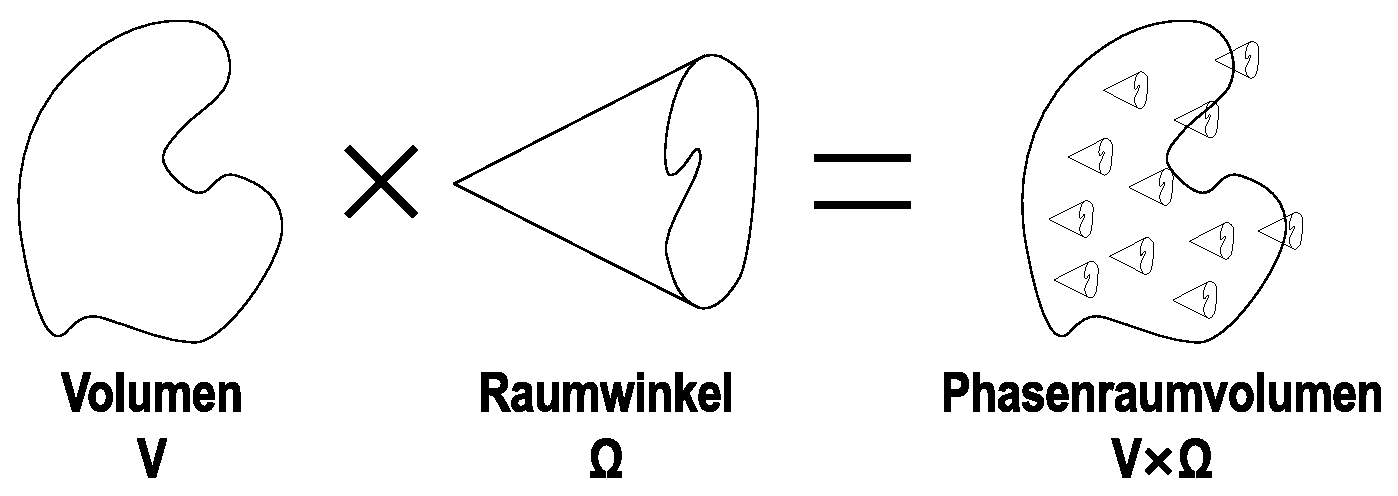
\includegraphics[width=0.8\textwidth]{phasespacevolume.eps}
		\caption{Darstellung einer Teilmenge $V \times \Omega$ des Phasenraums. Sie repr"asentiert alle Teilchen die sich innerhalb des Volumens $V$ befinden und sich in eine Richtung innerhalb von $\Omega$ bewegen.}
		\label{fig:phasespacevolume}
	\end{figure}

	Zur {\em Emission} z"ahlt jeder Prozess der neue Teilchen erzeugt. Dies kann durch verschiedene physikalische Prozesse, wie z.B. chemische Reaktionen, thermische Emission oder Kernfusion begr"undet sein. Emission innerhalb von $V$ in eine Richtung innerhalb von $\Omega$ ver"andert also die Teilchenbilanz, da sie eine Quelle f"ur Teilchen darstellt. Nach der Emission bewegen sich die Teilchen in unserem Modell gradlinig mit konstanter Geschwindigkeit bis sie eine instantane Kollision mit dem Medium erfahren. Bewegt sich ein Teilchen bei seiner gradlinigen Bewegung in das Volumen $V$ hinein oder aus ihm heraus und bewegt es sich dabei in eine Richtung innerhalb von $\Omega$, so "andert das ebenfalls unsere Teilchenbilanz. In diesem Fall sprechen wir von {\em Durchstr"omen}. Findet als letzte M"oglichkeit eine {\em Kollision} des Teilchens mit dem Medium innerhalb von $V$ statt, kann das Teilchen entweder absorbiert oder gestreut werden. Wird es absorbiert wirkt dies als Teilchensenke. Wird es gestreut, dann kann es, je nachdem in welche Richtung es sich vor und nach der Kollision bewegt hat, entweder keinen Einflu"s auf die Teilchenbilanz haben (Bewegungsrichtung vor und nach der Kollision entweder innerhalb oder ausserhalb von $\Omega$), es kann herausgestreut werden (Bewegungsrichtung vor der Kollision innerhalb und nach der Kollision ausserhalb von $\Omega$) oder aber hineingestreut werden (Bewegungsrichtung vor der Kollision ausserhalb und nach der Kollision innerhalb von $\Omega$) werden.
	
	Um die einzelnen Beitr"age dieser Prozesse zur Teilchenbilanz quantitativ zu erfassen f"uhren wir die Teilchenzahl $$N(t):=\int_\Omega \int_V n(\location{r},\omega,t)\,d\location{r}\,d\omega$$ ein. Sie gibt an wieviele Teilchen sich zum Zeitpunkt $t$ im Phasenraumvolumen $V \times \Omega$ befinden. Durch die eben beschriebenen Prozesse "andert sich $N(t)$ normalerweise mit der Zeit. Ist die Zeit, die ein Teilchen ben"otigt das betrachtete System zu durchqueren, klein gegen"uber der typischen Zeitskala, nach der sich das System bedeutend ver"andert hat, k"onnen wir annehmen, da"s sich die Teilchenzahl f"ur jedes Phasenraumvolumen im dynamischen Gleichgewicht befindet, d.h. das zwar st"andig Teilchen aus dem Phasenraumvolumen hinein- und hinausstr"omen, erzeugt, absorbiert und gestreut werden, aber sich alle Prozesse in der Bilanz die Waage halten, $N(t)$ also station"ar ist:$$\frac{dN(t)}{dt}=0\qquad\left[\frac{1}{\text{s}}\right].$$ Teilen wir diese "Anderung von $N$ mit der Zeit auf die verschiedenen obengenannten Prozessen auf sind wir bei der Grundlage einer Bilanzgleichung angelangt:$$\begin{bmatrix}\text{"Anderung}\\ \text{durch}\\ \text{Emission}\end{bmatrix}+\begin{bmatrix}\text{"Anderung}\\ \text{durch}\\ \text{Durchstr"omung}\end{bmatrix}+\begin{bmatrix}\text{"Anderung}\\ \text{durch}\\ \text{Kollisionen}\end{bmatrix}=0.$$ Wir leiten nun f"ur jeden dieser Ausdr"ucke einen Formelausdruck her.
	Die "Anderung aufgrund von Emission nennen wir $$\mathbf{E}=\int_\Omega \int_V q(\location{r},\omega)\,d\location{r}\,d\omega\qquad\left[\frac{1}{\text{s}}\right],$$ wobei wir die Phasenraumquellfunktion $q$ (mit Einheit $\text{m}^{-3}\text{sr}^{-1}\text{s}^{-1}$) eingef"uhrt haben, die f"ur jeden Ort $\location{r}$ und jede Raumrichtung $\omega$ die Anzahl erzeugter Teilchen pro Sekunde, Einheitsvolumen und Einheitsraumwinkel angibt. Hinein- und herausstr"omende Teilchen erzeugen eine Teilchenrate
	$$\mathbf{S}=\int_\Omega \int_{\partial V} \phi(\location{s},\omega)(\omega \cdot d\location{s})d\omega,$$
	die wir durch Integrieren "uber $\partial V$ (die Oberfl"ache von V) erhalten. Hierbei steht $\location{s}$ f"ur ein infinitesimales als Vektor repr"asentiertes Fl"achenelement, dessen Richtung die Fl"achennormale, und dessen L"ange seine Fl"ache repr"asentiert. Das Skalarprodukt zwischen Bewegungsrichtung $\omega$ und Fl"achennormalen sorgt f"ur das richtige Vorzeichen, wobei ein positiver Wert Teilchenverlust bedeutet.
	Der letzte Beitrag $\mathbf{C}$ tr"agt den Kollisionen Rechnung. Da Teilchen nur mit dem Medium nicht aber untereinander interagieren mu"s die Kollisionsrate unabh"angig von $\phi$ sein. Wir unterteilen $\mathbf{C}$ in einen Absorptionsteil $\mathbf{C}_\text{abs}$ und einen Streuanteil $\mathbf{C}_\text{sca}$. Wir nehmen an, da"s die Wahrscheinlichkeit, da"s ein Teilchen aufgrund von Absorption verschwindet proportional zur zur"uckgelegten Distanz im Medium, nicht aber von der Bewegungsrichtung durch das Medium ist (was gleichbedeutend mit der Annahme eines isotropen Mediums ist). Die Proportionalit"atskonstante am Ort $\location{r}$ nennen wir den (Volumen-)Absorptionsquerschnitt $\kappa(\location{r})$ ($[\kappa]=\frac{1}{\text{m}}=\frac{m^2}{m^3}$). Die zugeh"orige Teilchenrate ist
	$$\mathbf{C}_\text{abs}=\int_\Omega \int_V \kappa(\location{r})\phi(\location{r},\omega)\,d\location{r}\,d\omega.$$
	Die genauen Mechanismen der Streuung k"onnen durch Mie--Theorie oder Quantenmechanik behandelt werden. In unserem Teilchentransport repr"asentieren wir diese Streumodelle durch die Streuphasenfunktion $k(\location{r},\omega,\omega')$ und den Volumenstreuquerschnitt $\sigma(\location{r})$. Dabei gibt $k(\location{r},\omega,\omega')$ bei Streuung eines aus Richtung $\omega$ kommenden Teilchens am Ort $\location{r}$ die Wahrscheinlichkeit pro Einheitsraumwinkel an, nach $\omega'$ gestreut zu werden. Da ein gestreutes Teilchen irgendwohin gestreut wird, gilt f"ur $k$ die Normierungsbedingung
	\begin{equation}\label{eq:k_norm_req}
	  \int_{\mathcal{S}^2} k(\location{r},\omega,\omega')\,d\omega'=1.
	\end{equation}
	Ausserdem ist $k$ symmetrisch bez"uglich der Vertauschung der Bewegungsrichtungen vor und nach der Streuung:
	$$k(\location{r},\omega,\omega')=k(\location{r},\omega',\omega)\quad \forall\:\omega,\omega'\in\mathcal{S}^2.$$
	Beide Bedingungen werden z.B. durch die isotrope Streuphasenfunktion $$k_\text{iso}(\location{r},\omega,\omega')=\frac{1}{4\pi}$$ erf"ullt.
	Wie bei der Absorption, nehmen wir an, da"s die Wahrscheinlichkeit eines Teilchens gestreut zu werden von der durch das Medium zur"uckgelegten Distanz, nicht aber von der Bewegungsrichtung abh"angt. Wir teilen $\mathbf{C}_\text{sca}$ weiter auf, in einen Teil
	$$\mathbf{C}_\text{out}=\int_\Omega \int_V \int_{\mathcal{S}^2} \sigma{(\location{r})}k(\location{r},\omega,\omega')\phi(\location{r},\omega)\,d\omega'\,d\location{r}\,d\omega,$$
	der herausgestreute Teilchen ber"ucksichtigt, sowie einen Teil
	$$\mathbf{C}_\text{in}=\int_\Omega \int_V \int_{\mathcal{S}^2} \sigma{(\location{r})}k(\location{r},\omega',\omega)\phi(\location{r},\omega')\,d\omega'\,d\location{r}\,d\omega$$
	entsprechend f"ur hineingestreute Teilchen. Dabei sollte erw"ahnt werden, da"s sowohl $\mathbf{C}_\text{out}$ als auch $\mathbf{C}_\text{in}$ Teilchen ber"ucksichtigen, deren Richtung vor und nach der Streuung in $\Omega$ liegt, was weder einem Zuwachs noch einem Verlust an Teilchen entspricht. Da f"ur unsere Bilanz aber immer nur die Differenz von $\mathbf{C}_\text{out}$ und $\mathbf{C}_\text{in}$ betrachtet wird, hebt sich dieser Teil wieder heraus. Alternativ k"onnten wir auch "uber $\mathcal{S}^2 \setminus \Omega$ integrieren, was zu einer komplizierteren Rechnung, aber zu keinem anderen Endergebnis f"uhren w"urde. F"ugen wir die Einzelterme zusammen und ordnen nach Zuw"achsen und Verlusten sieht unsere Bilanzgleichung f"ur die Teilchenraten in $V \times \Omega$ wie folgt aus:
	$$\underbrace{\mathbf{S}+\mathbf{C}_\text{abs}+\mathbf{C}_\text{out}}_\text{Verluste}=\underbrace{\mathbf{E}+\mathbf{C}_\text{in}}_\text{Zuw"achse}$$
	Es f"allt bei der Betrachtung der Formeln f"ur die einzelnen Terme auf, da"s alle Terme, bis auf $\mathbf{S}$ Volumenintegrale "uber $V$ enthalten. $\mathbf{S}$ enth"alt stattdessen ein Oberfl"achenintegral "uber $\partial V$. Mithilfe des Gauss'schen Satzes dr"ucken wir das Oberfl"achenintegral "uber $\partial V$ durch ein Volumenintegral "uber $V$ aus und erhalten
	$$\mathbf{S}=\int_\Omega \int_V \omega \cdot (\nabla\phi)(\location{r},\omega)\,d\location{r}\,d\omega,$$
	wobei wir $\nabla \cdot(\omega\phi)=\omega\cdot(\nabla\phi)$ benutzt haben.
	
	In unserer Bilanzgleichung treten jetzt nur noch Volumenintegrale "uber unser Phasenraumvolumen $V \times \Omega$ auf. Da $V$ und $\Omega$ beliebig gew"ahlt waren, mu"s die Bilanzgleichung "uberall und in alle Richtungen lokale G"ultigkeit haben:
	\begin{multline*}
	  \omega\cdot\nabla\phi(\location{r},\omega)+\kappa(\location{r})\phi(\location{r},\omega)+\int_{\mathcal{S}^2}\sigma(\location{r})k(\location{r},\omega,\omega')\phi(\location{r},\omega)d\omega' \\
	  =q(\location{r},\omega)+\int_{\mathcal{S}^2}\sigma(\location{r})k(\location{r},\omega',\omega)\phi(\location{r},\omega')d\omega'
	\end{multline*}
	Da beim $\mathbf{C}_\text{out}$--Integral $\sigma$ und $\phi$ nicht von der Integrationsvariable abh"angen und das verbleibende Integral aufgrund der Normierungsbedingung (\ref{eq:k_norm_req}) gleich eins ist vereinfacht sich unsere Bilanzgleichung schlu"sendlich zu
	\begin{equation}\label{eq:particle_balance_equation}
	  \omega\cdot\nabla\phi(\location{r},\omega)+\left(\kappa(\location{r})+\sigma(\location{r})\right)\phi(\location{r},\omega)
	  =q(\location{r},\omega)+\sigma(\location{r})\int_{\mathcal{S}^2}k(\location{r},\omega',\omega)\phi(\location{r},\omega')d\omega'
	\end{equation}
	Die Bilanzgleichung hat die Gestalt einer Integro--Differentialgleichung in $\phi$.
	Im folgenden Abschnitt stellen wir den Bezug zwischen unseren abstrakten Teilchentransportgr"o"sen und physikalischen Strahlungsgr"o"sen her.

	\section{Ph"anomenologische Strahlungsgr"o"sen}\label{subsec:strahlungsgroessen}
	Im vorigen Abschnitt haben wir das Strahlungstransportproblem bewu"st auf ein Teilchentransportproblem mit abstrakten Teilchen statt Photonen reduziert um einerseits eine klarere Herleitung zu erm"oglichen und um andererseits die Verwandtschaft zu anderen Transportproblemen (wie z.B. Neutronentransport) offensichtlich zu machen. Um nun den Anschlu"s zu radiometrischen Strahlungsgr"o"sen zu bekommen, ersetzen wir unsere abstrakten Teilchen wieder durch Photonen. Photonen haben u.a. zwei Eigenschaften die wir daher ber"ucksichtigen. Sie bewegen sich konstant mit Lichtgeschwindigkeit, d.h. wir k"onnen die vorher gebrauchte allgemeine Teilchengeschwindigkeit $v$ gleich $\text{c}$ setzten. Ausserdem besitzt jedes Photon eine Energie, die durch seine Frequenz $\nu$ mit 
	$$E=h\nu \qquad[J]$$
	bestimmt ist. Dabei bezeichnet $h$ das Planck'sche Wirkungsquantum.
	Jeder Frequenz $\nu$ k"onnen wir ein monochromatisches Transportproblem zuordnen, dessen L"osung in Form eines Phasenraumflusses $\phi_\nu$ die Photonenfrequenz als Index tr"agt.
	Die {\em spezifische Intensit"at} $I_\nu(\location{r},\omega)$ erhalten wir nun aus dem Phasenraumflu"s bzw. der Phasenraumdichte gem"a"s
	\begin{align}\label{eq:intensity_def}
		I_\nu(\location{r},\omega)d\nu & = h\nu\,\phi_\nu(\location{r},\omega)\\
		                       & = c h\nu\,n_\nu(\location{r},\omega) \qquad \left[\frac{\text{W}}{\text{m}^2\text{sr}}\right] \nonumber
	\end{align}
	Sie gibt an, wieviel Joule am Ort $\location{r}$ pro Sekunde durch eine Einheitsfl"ache mit Fl"achennormale $\omega$ pro Einheitsraumwinkel in Richtung $\omega$ und pro Frequenzintervall durch Photonen mit Frequenz $\nu$ transportiert wird:
	$$dE_\nu=I_\nu(\location{r},\omega) dA\,dt\,d\omega\,d\nu.$$
	Wir f"uhren au"serdem die {\em spezifische Emissivit"at} $\varepsilon_\nu$ ein. Wir erhalten Sie aus der Phasenraumquellfunktion $q_\nu$ durch
	\begin{equation}\label{eq:emissivity_def}
		\varepsilon_\nu(\location{r},\omega)d\nu = h\nu\,q_\nu(\location{r},\omega) \qquad \left[\frac{\text{W}}{\text{m}^3\text{sr}}\right].
	\end{equation}
	
	Multiplizieren wir unsere abstrakte Transportgleichung (\ref{eq:particle_balance_equation}) mit $h\nu$ und benutzen wir die Beziehungen (\ref{eq:intensity_def},\ref{eq:emissivity_def}) erhalten wir mit
	\begin{equation}\label{eq:stg_diff}
	  \omega\cdot\nabla I_\nu(\location{r},\omega)+\left(\kappa_\nu(\location{r})+\sigma_\nu(\location{r})\right)I_\nu(\location{r},\omega)
	  =\varepsilon_\nu(\location{r},\omega)+\sigma_\nu(\location{r})\int_{\mathcal{S}^2}k_\nu(\location{r},\omega',\omega)I_\nu(\location{r},\omega')d\omega'
	\end{equation}
	die {\em Strahlungstransportgleichung in differentieller Form}. Sie stellt eine Integro--Differentialgleichung f"ur $I_\nu$ auf unserem 5--dimensionalen Phasenraum $\mathbb{R}^3 \times \mathcal{S}^2$ dar und kann f"ur jede Frequenz $\nu$ getrennt gel"ost werden. Sie gibt f"ur jede Kombination aus Ort $\location{r}$ und Photonen--Ausbreitungsrichtung $\omega$ das lokal zu erf"ullende Gleichgewicht aus Verlusten (linke Seite) und Zuw"achsen (rechte Seite) an.
	
	Wir fassen die Verluste durch Absorption und Streuung mit dem {\em Vo\-lu\-men\-ex\-tink\-ti\-ons\-quer\-schnitt}
	$$\xi_\nu(\location{r}):=\kappa_\nu(\location{r})+\sigma_\nu(\location{r}) \qquad\left[\frac{1}{m}\right]$$
	zusammen, wodurch wir (\ref{eq:stg_diff}) auch als
	\begin{equation}\label{eq:stg_diff2}
	  \omega\cdot\nabla I_\nu(\location{r},\omega)+\xi_\nu(\location{r})I_\nu(\location{r},\omega)
	  =\varepsilon_\nu(\location{r},\omega)+\sigma_\nu(\location{r})\int_{\mathcal{S}^2}k_\nu(\location{r},\omega',\omega)I_\nu(\location{r},\omega')d\omega'
	\end{equation}
	schreiben k"onnen.
	Ausserdem definieren wir die dimensionslose {\em optische Tiefe}
	\begin{equation*}
		\tau_\nu(\location{r}_1,\location{r}_2):=\int_{s=0}^{||\location{r}_2-\location{r}_1||} \xi_\nu(\location{r}_1+s(\location{r}_2 - \location{r}_1))\,ds,
	\end{equation*}
	die ein Ma"s f"ur die Undurchsichtigkeit des Mediums bei der Frequenz $\nu$ zwischen zwei Orten $\location{r}_1$ und $\location{r}_2$ ist. Nehmen wir uns Gleichung (\ref{eq:stg_diff2}), betrachten nur die Verluste (indem wir die rechte Seite zu Null setzen) und w"ahlen eine beliebige Richtung $\omega$, gelangen wir zur gew"ohnlichen Differentialgleichung
	$$I_\nu'(s)+\xi_\nu(s)I_\nu(s)=0$$
	die durch
	$$I_\nu(s)=I_\nu(0)\:\text{exp}\left(-\int_{s'=0}^s \xi_\nu(s')\right)=I_\nu(0)\:\text{exp}\left(-\tau_\nu(0,s)\right)$$
	gel"ost wird. Die L"osung zeigt, da"s die optische Tiefe zu einer exponentiellen Abschw"achung der Intensit"at f"uhrt.
	
	
	\section{Die Messgleichung}
	Mit dem Strahlungsintensit"atsfeld, da"s aus der Gesamtheit aller spezifischen Intensit"aten $I_\nu$ besteht, meinen wir die Funktion
	$$I:\mathbb{R}_{\geq 0}\times\mathbb{R}^3\times\mathcal{S}^2\to\mathbb{R}_{\geq 0}\;,\qquad (\nu,\location{r},\omega)\mapsto I_\nu(\location{r},\omega),$$
	die vom 6--dimensionalen Raum aller Photonenfrequenzen, Orte und Raumrichtungen auf die dort herrschende spezifische Intensit"at abbildet.
	
	Funktionen dieser Art bilden einen Skalarproduktraum. Das Null--Element ist die konstant auf Null abbildende Funktion. Zwei Funktionen lassen sich punktweise addieren und ergeben so eine neue Funktion die auch nach $\mathbb{R}_{\geq 0}$ abbildet. Das Skalarprodukt zwischen zwei Funktionen $f$ und $g$ ist schlie"slich mit
	$$\langle f,g\rangle=\int_{\mathbb{R}_{\geq 0}} \int_{\mathbb{R}^3} \int_{\mathcal{S}^2} f(\nu,\location{r},\omega)g(\nu,\location{r},\omega)\,d\omega\,d\location{r}\,d\nu$$
	gegeben.
	
	Mit diesem funktionalanalytischem Handwerkszeug definieren wir eine Messung als das Skalarprodukt zwischen unserem Strahlungsintensit"atsfeld $I$ und einer {\em Sensitivit"atsfunktion} $W$, welche die St"arke der Gewichtung angibt, mit der die spezifische Intensit"at der Frequenz $\nu$ am Ort $\location{r}$ in Richtung $\omega$ in den Me"swert eingeht. Die entsprechende Formel
	\begin{equation}\label{eq:messgleichung}
		M^{(i)}:=\langle W^{(i)},I\rangle=\int_{\mathbb{R}_{\geq 0}} \int_{\mathbb{R}^3} \int_{\mathcal{S}^2} W^{(i)}(\nu,\location{r},\omega)I_\nu(\location{r},\omega)\,d\omega\,d\location{r}\,d\nu
	\end{equation}
	nennen wir {\em Me"sgleichung} (f"ur den $i$--ten Sensor). F"ur monochromatische Messungen f"uhren wir zus"atzlich noch 
	\begin{equation}\label{eq:messgleichung_mono}
		M_\nu^{(i)}:=\langle W_\nu^{(i)},I_\nu\rangle=\int_{\mathbb{R}^3} \int_{\mathcal{S}^2} W_\nu^{(i)}(\location{r},\omega)I_\nu(\location{r},\omega)\,d\omega\,d\location{r}
	\end{equation}
	ein, womit wir (\ref{eq:messgleichung}) auch als
	\begin{equation}\label{eq:messgleichung_frommonos}
		M^{(i)}=\int_{\mathbb{R}_{\geq 0}} M_\nu^{(i)}\,d\nu
	\end{equation}
	schreiben k"onnen
	Die Tatsache, da"s wir die Sensitivit"atsfunktion nicht n"aher spezifizieren, erlaubt uns die gr"o"stm"ogliche Freiheit beim kreieren virtueller Sensoren. Beispielsweise k"onnte $W$ nur f"ur einen kleines Volumen und einen kleinen Raumwinkel aber bei allen Frequenzen nichtverschwindend sein, und so einen virtuellen Sensor zur Messung der Gesamt--Intensit"at an einem bestimmten Ort in eine bestimmte Richtung repr"asentieren. Ebenso kann durch gleichstarke Gewichtung aller Raumrichtungen die mittlere Intensit"at gemessen werden.
	
	Was hier vielleicht als ein nur theoretisch interessantes Konstrukt ohne praktischen Nutzen erscheint, erweist sich sp"ater insbesondere in Verbindung mit Monte--Carlo--Sampling als ein gleichzeitig vielseitiges und effizientes Werkzeug.	
	
	
	\section{"Ubersicht etablierter L"osungsverfahren}
	TODO: "Ubersicht benutzter L"osungsverfahren, Meilensteine (wann zum ersten mal Polarisation gerechnet?, Warum etablieren sich MC-Verfahren so sp"at?, etc...)
		
	\chapter{Pfadintegralformulierung der Strahlungstransportgleichung}
	In diesem Abschnitt leiten wir eine alternative mathematische Formulierung der Strahlungstransportgleichung einerseits und ihrer L"osung (genau genommen, Messungen der L"osung im Sinne von (\ref{eq:messgleichung})) andererseits her. Dies f"uhrt uns durch die verschiedenen, auf das Problem eingenommenen Blickwinkel, zu einem besseren Verst"andnis von Strahlungstransport und gibt uns dar"uber hinaus einen neuen Ansatzpunkt zur effizienten L"osung des Strahlungstransportproblems.
	
	Die Idee zu dieser Formulierung kommt aus der Dissertation von \citet{Veach:1997p9136}, wird aber schon in \citep{Arvo:1995p9257} vorgestellt. Beide Dissertationen behandeln allerdings nur den Strahlungstransport zwischen Oberfl"achen. In der Arbeit von \citet{Pauly:2000p5705} wird dies auf partizipierende Medien ausgedehnt. Aus \citep{Arvo:1993p9035} stammt ausserdem die Herleitung der integralen Form der Strahlungstransportgleichung.
	
	
	\section{Strahlungstransportgleichung in integraler Form}
	In differentieller Form nimmt die Strahlungstransportgleichung, wie wir in Abschnitt (\ref{subsec:strahlungsgroessen}) gesehen haben, folgende Gestalt an:
		\begin{equation}
			\omega \cdot \nabla I(\location{r},\omega)+\overbrace{\left(\kappa(\location{r})+\sigma(\location{r})\right)}^{=:\xi(\location{r})}I(\location{r},\omega)=\varepsilon(\location{r},\omega)+\sigma(\location{r}) \int_{\mathcal{S}^2} k(\location{r},\omega',\omega)I(\location{r},\omega') d\omega'.
			\label{eq:diff.STG}
		\end{equation}
	F"ur diesen und die folgenden Abschnitte lassen wir dabei den Index $\nu$ aus "Ubersichtsgr"unden weg, womit gemeint ist, da"s wir stellvertretend f"ur alle Frequenzen ein einzelnes monochromatisches Strahlungstransportproblem einer beliebigen Frequenz nehmen. Wenn wir zum polychromatischen Fall zur"uckkehren f"uhren wir die Indizes wieder ein.
	
	Schreiben wir das Skalarprodukt zwischen $\omega$ und dem $\nabla$--Operator als Richtungsableitung
	\newcommand{\dds}{\frac{\text{d}}{\text{d}s}}
	\newcommand{\ddszero}{\left. \dds \right|_{s=0}}
	\begin{equation*}
		\omega \cdot \nabla I(\location{r},\omega)
		=  \ddszero I(\location{r}+s\,\omega,\omega)
		=  -\ddszero I(\location{r}-s\,\omega,\omega)
	\end{equation*}
	k"onnen wir (\ref{eq:diff.STG}) als
	\begin{multline}
		\dds I(\location{r}-s\,\omega,\omega) - \xi(\location{r}-s\,\omega)I(\location{r}-s\,\omega,\omega) = \\-\varepsilon(\location{r}-s\,\omega,\omega) -\sigma(\location{r}-s\,\omega) \int_{\mathcal{S}^2} k(\location{r}-s\,\omega,\omega',\omega)I(\location{r}-s\,\omega,\omega') \text{d}\omega'
		\label{eq:diff.STGtranslated}
	\end{multline}
	umschreiben. Dabei haben wir die Beschr"ankung $s=0$ fallengelassen, was die Korrektheit der Umformung aber nicht "andert. Mit den Abk"urzungen
	\begin{align*}
		{\hat I}(s)&:=I(\location{r}-s\,\omega,\omega) \\
		Q(\location{r},\omega)&:= \varepsilon(\location{r},\omega)+\sigma(\location{r}) \int_{\mathcal{S}^2} k(\location{r},\omega',\omega)I(\location{r},\omega') d\omega' \\
		{\hat Q}(s)&:=Q(\location{r}-s\,\omega,\omega)\\
		{\hat \xi}(s)&:=\xi(\location{r}-s\,\omega) \\
		{\hat \tau}(s)&:= \int_{s'=0}^{s} {\hat \xi}(s') \text{d}s'
	\end{align*}
	wird aus (\ref{eq:diff.STGtranslated})
	\begin{equation}
		\dds {\hat I}(s) - {\hat \xi}(s){\hat I}(s)= -{\hat Q}(s) \qquad |\cdot e^{-{\hat \tau}(s)}.
		\label{eq:diff.STGhatted}
	\end{equation}
	Gleichung (\ref{eq:diff.STGhatted}) ist eine gew"ohnliche Differentialgleichung die sich mit
	\begin{align}
		(\ref{eq:diff.STGhatted})\Leftrightarrow\qquad \dds \left(e^{-{\hat \tau}(s)} {\hat I}(s)\right)&= -e^{-{\hat \tau}(s)} {\hat Q}(s) \qquad | \int_{s'=0}^s (\cdot)\text{d}s' \nonumber \\
		\Leftrightarrow\qquad e^{-{\hat \tau}(s)} {\hat I}(s) - {\hat I}(0) &= -\int_{s'=0}^s e^{-{\hat \tau}(s')} {\hat Q}(s') \text{d}s' \nonumber \\
		\Leftrightarrow\qquad {\hat I}(0) &= e^{-{\hat \tau}(s)} {\hat I}(s) + \int_{s'=0}^s e^{-{\hat \tau}(s')} {\hat Q}(s') \text{d}s' \label{eq:diff.STGpreintegral}
	\end{align}
	leicht nach ${\hat I}(0)$ aufl"osen l"asst. Obwohl ${\hat Q}(s)$ lokal die Intensit"at $I$ "uber alle Raumrichtungen integriert, d"urfen wir f"ur die L"osung von (\ref{eq:diff.STGhatted}) $Q$ als unabh"angig von $I$ behandeln, da die Schnittmenge zwischen der Geraden im Raum, auf der wir die Differentialgleichung l"osen, und der Menge aller Raumrichtungen $\mathcal{S}^2$ bei der Integration "uber alle Raumrichtungen eine Nullmenge ist und somit f"ur physikalisch relevante Strahlungsintensit"atsfelder (d.h. solche, die hinreichend stetig/beschr"ankt bzw. keine Delta--Distribution sind) keinen Beitrag zum Integral leistet.
	Setzen wir in (\ref{eq:diff.STGpreintegral}) f"ur die Abk"urzungen wieder die urspr"unglichen Ausdr"ucke ein, erhalten wir die {\em Strahlungstransportgleichung in integraler Form}:
	\begin{multline}
		I(\location{r},\omega) = e^{-\tau(\location{r},\location{r}-s\,\omega)} {\hat I}(\location{r},\location{r}-s\,\omega) + \int_{s'=0}^\infty e^{-\tau(\location{r},\location{r}-s\,\omega)} \;\cdot \\
		\quad\cdot\left( \varepsilon(\location{r}-s'\,\omega,\omega) + \sigma(\location{r}-s'\,\omega)
		\left[ \int_{\mathcal{S}^2} k(\location{r}-s'\,\omega,\omega',\omega)I(\location{r}-s'\,\omega,\omega') \text{d}\omega'\right] \right) \text{d}s'
		\label{eq:int.STG}
	\end{multline}
	Nehmen wir nun als Randbedingungen an, da"s in unendlich gro"ser Entfernung keine Lichtquellen existieren, d.h. $\forall \omega \in \mathcal{S}^2 : I(\location{r}=-\infty\cdot\omega,\omega)=0$, dann vereinfacht sich (\ref{eq:int.STG}) zu
	\begin{multline}
		I(\location{r},\omega) = \int_{s'=0}^\infty e^{-\tau(\location{r},\location{r}-s\,\omega)} \;\cdot \\
		\quad\cdot\left( \varepsilon(\location{r}-s'\,\omega,\omega) + \sigma(\location{r}-s'\,\omega)
		\left[ \int_{\mathcal{S}^2} k(\location{r}-s'\,\omega,\omega',\omega)I(\location{r}-s'\,\omega,\omega') \text{d}\omega'\right] \right) \text{d}s'
		\label{eq:int.STGdarkbg}
	\end{multline}


	\section{Strahlungstransportgleichung in Operator--Form}
	Schauen wir uns die einzelnen Teile der Gleichung (\ref{eq:int.STGdarkbg}) genauer an.
	Der innere Teil von (\ref{eq:int.STGdarkbg}) in eckigen Klammern summiert an einem festen Ort ($\location{r}-s'\,\omega$), mit der Streuphasenfunktion $k$ gewichtet, die einfallenden Intensit"aten auf, die in Richtung $\omega$ gestreut werden. Anschliessend skaliert der Volumenstreuquerschnitt die aufintegrierte Intensit"at entsprechend dem lokal vorhandenen Medium und gibt dabei dem Ausdruck die Einheit einer Emissivit"at.
	Der restliche "aussere Teil der Gleichung addiert die eben gewonnene Emissivit"at durch Einstreuung zu der lokal durch Ausstrahlung erzeugten Emissivit"at an jedem Punkt auf einer Geraden hinter dem Punkt $\location{r}$ und summiert, die mit einem der optischen Tiefe entsprechenden Abschw"achungsfaktor gewichteten, in Richtung $\omega$ zeigenden, Emissivit"aten, entlang der Geraden zur Gesamtintensit"at am Ort $\location{r}$ in Richtung $\omega$ auf.
	Der Gesamtausdruck l"asst sich durch Einf"uhrung zweier neuer Operatoren
	\begin{align*}
		\left(\mathbf{G}\varepsilon\right)(\location{r},\omega)&:=\int_{s'=0}^\infty e^{-\tau(\location{r}-s' \omega,\location{r})}\varepsilon(\location{r}-s' \omega,\omega) ds' \\
		\left(\mathbf{K}I\right)(\location{r},\omega)&:=\sigma(\location{r})\int_{S^2} k(\location{r},\omega',\omega) I(\location{r},\omega') d\omega'
	\end{align*}
	\begin{equation*}
		\mathbf{G} : \varepsilon(\location{r},\omega) \mapsto I(\location{r},\omega) , \qquad
		\mathbf{K} : I(\location{r},\omega) \mapsto \varepsilon(\location{r},\omega)
	\end{equation*}
	in elementarere Prozesse aufteilen. Wir nennen $\mathbf{G}$ den sogenannten {\em Fortpflanzungs--Operator} und $\mathbf{K}$ den {\em Streu--Operator}. Beides sind Integraloperatoren auf dem Raum der Funktionen $f : \mathbb{R}^3 \times \mathcal{S}^2 \to \mathbb{R}_{\geq 0}$, die vom Teilchen--Phasenraum auf die positiven reellen Zahlen abbilden. Beide haben komplement"are Lokalit"aten. W"ahrend $\mathbf{K}$ lokal im Ort "uber alle Raumrichtungen integriert, ist $\mathbf{G}$ lokal in der Raumrichtung und integriert "uber alle Orte entlang einer Geraden im Raum. Dabei bildet $\mathbf{K}$ von einem Strahlungsintensit"atsfeld auf ein Emissivit"atsfeld ab. Bei $\mathbf{G}$ ist es umgekehrt, es macht aus einem Emissivit"atsfeld wieder ein Strahlungsintensit"atsfeld.
	Mit diesen neuen Operatoren wird aus Gleichung (\ref{eq:int.STGdarkbg}) die {\em Operatorform der Strahlungstransportgleichung}
	\begin{equation}
		I=\mathbf{G}(\varepsilon + \mathbf{K}I),
		\label{eq:op.STG}
	\end{equation}
	die wir nach $I$ aufl"osen k"onnen:
	\begin{align}
		(\ref{eq:op.STG}) \Leftrightarrow I&=\mathbf{G}\varepsilon + \mathbf{GK}I \nonumber \\
		\Leftrightarrow (\mathbf{1}-\mathbf{GK})I &= \mathbf{G}\varepsilon \nonumber \\
		\Leftrightarrow I &= (\mathbf{1}-\mathbf{GK})^{-1}\mathbf{G}\varepsilon \label{eq:op.STGinvert} \\
		\Leftrightarrow I &= \sum_{k=0}^\infty (\mathbf{GK})^k \mathbf{G}\varepsilon \label{eq:op.STGneumann} \\
		&=\mathbf{G}\varepsilon + \mathbf{GKG}\varepsilon + \mathbf{GKGKG}\varepsilon + \hdots \label{eq:op.STGneumann.explicit} \\
		\Leftrightarrow I &=\sum_{k=0}^\infty \mathbf{G} (\mathbf{KG})^k \varepsilon \label{eq:op.STGkg}
	\end{align}
	Damit ist das Strahlungstransportproblem formal gel"ost! Dabei haben wir den auftretenden invertierten Operator (\ref{eq:op.STGinvert}) durch eine Neumann--Reihe (\ref{eq:op.STGneumann}) ersetzt. Dies ist dann zul"assig wenn die Operatornorm des Operators $\mathbf{GK}$ kleiner als eins ist und damit sichergestellt ist, da"s die Neumann--Reihe konvergiert. F"ur alle praktisch relevanten Probleme ist dies der Fall \citep[siehe][Theorem 12 und 13]{Arvo:1995p9257}. Physikalisch l"asst sich das Gleichgewichts--Strahlungsintensit"atsfeld als Summe aus Intensit"atsfeldern verstehen, die durch Photonen mit unterschiedlich vielen Streuereignissen auf ihrem Weg von der Emission aus einer Lichtquelle bis zu ihrer Messung mit einem Me"sinstrument entstanden sind (wie in Schritt (\ref{eq:op.STGneumann.explicit}) deutlich wird). Dabei m"ussen Pfade jeder m"oglichen L"ange (sprich Anzahl an Streuereignissen) ber"ucksichtigt werden. Zwischen Emission und Messung wechseln sich dabei Fortpflanzung $\mathbf{G}$ und Streuung $\mathbf{K}$ ab. Im letzen Schritt (\ref{eq:op.STGkg}) haben wir $\mathbf{G}$ nach links ausgeklammert um den $\mathbf{KG}$--Operator herauszustellen.
	
	
	\section{KG--Operator in Volumenform}
	Schauen wir uns den $\mathbf{KG}$--Operator genauer an. $\mathbf{KG}$ bildet ein Emissivit"atsfeld nach Fortpflanzung und Aufintegration zu einem Intensit"atsfeld und anschliessender Streuung auf ein neues Emissivit"atsfeld ab:
	\begin{equation*}
		\mathbf{KG} : \varepsilon(\location{r},\omega) \mapsto \varepsilon(\location{r},\omega)
	\end{equation*}

	Setzen wir die Definitionen der Operatoren ein und formen ein wenig um:
	\begin{align*}
		\left(\mathbf{KG}\varepsilon\right)(\location{r},\omega)&=\sigma(\location{r}) \int_{\mathcal{S}^2} k(\location{r},\omega',\omega)\left[\int_{s'=0}^\infty e^{-\tau(\location{r}-s' \omega',\location{r})}\varepsilon(\location{r}-s' \omega',\omega') \text{d}s'\right] \text{d}\omega' \\
		&=\sigma(\location{r}) \int_{\mathcal{S}^2} \int_{s'=0}^\infty k(\location{r},\omega',\omega) e^{-\tau(\location{r}-s' \omega',\location{r})}\varepsilon(\location{r}-s' \omega',\omega') \underbrace{\text{d}s' \text{d}\omega'}_{=\frac{\text{d}\location{r}'}{s'^2}} \\
		&=\sigma(\location{r}) \int_{\mathbb{R}^3} k(\location{r},\omega',\omega) \frac{e^{-\tau(\location{r}',\location{r})}}{\|\location{r}-\location{r}'\|^2}\varepsilon(\location{r}',\omega') \,\text{d}\location{r}'
	\end{align*}
	Da wir durch Kombination der Integration "uber alle Raumrichtungen $\omega'$ und alle Entfernungen $s'$ den gesamten Raum abdecken, k"onnen wir die beiden Integrale zugunsten eines Volumenintegrals "uber den gesamten Raum sowie eines geometrischen Verd"unnungsfaktors tauschen. Mit dem Ziel, sp"ater alle Integrationen zu Volumenintegralen zusammenzufassen, schreiben wir den $\mathbf{KG}$--Operator so um, da"s alle expliziten Angaben von Entfernungen und Raumrichtungen durch eine raumpunktorientierte Notation ersetzt werden:
	\begin{multline}
		\left(\mathbf{KG}\varepsilon\right)(\location{r}_i \rightarrow\location{r}_{i+1})=\\
		\sigma(\location{r}_i) \int_{\mathbb{R}^3} k(\location{r}_{i-1}\rightarrow\location{r}_i\rightarrow\location{r}_{i+1})\frac{e^{-\tau(\location{r}_{i-1},\location{r}_i)}}{\|\location{r}_i-\location{r}_{i-1}\|^2}\varepsilon(\location{r}_{i-1} \rightarrow\location{r}_i)d\location{r}_{i-1}
		\label{eq:KGvolume_intermediate}
	\end{multline}
	Wir f"uhren zus"atzlich noch die Abk"urzung
	\begin{align*}
		\scatter{i}\;&:=\sigma(\location{r}_i)k(\location{r}_{i-1}\rightarrow\location{r}_i\rightarrow\location{r}_{i+1})\\
			&=\sigma(\location{r}_i)k(\location{r}_i,\normalized{\location{r}_i-\location{r}_{i-1}},\normalized{\location{r}_{i+1}-\location{r}_i})
	\end{align*}
	ein, soda"s wir (\ref{eq:KGvolume_intermediate}) zusammen mit den in Abschnitt \ref{subsec:nomenklatur} eingef"uhrten Schreibweisen noch kompakter als
	\begin{equation}
		\left(\mathbf{KG}\varepsilon\right)_{(i,i+1)}=\int_{\mathbb{R}^3} \scatter{i}\frac{e^{-\tau_{(i-1,i)}}}{d_{(i-1,i)}^2}\varepsilon_{(i-1,i)}d\location{r}_{i-1}.
		\label{eq:KGvolume}
	\end{equation}
	schreiben k"onnen.


	\section{Pfadintegrall"osung der Strahlungstransportgleichung}
	Wir setzen die Neumann--Reihen--L"osung (\ref{eq:op.STGkg}) in die monochromatische Me"sgleichung (\ref{eq:messgleichung_mono}) ein und erhalten
	\begin{align}
		M_\nu&=\int_{\mathbb{R}^3}\int_{\mathcal{S}^2}W_\nu(\location{r},\omega) \left(\sum_{k=0}^\infty \mathbf{G} (\mathbf{KG})^k \varepsilon_\nu\right)(\location{r},\omega) \,\text{d}\omega \,\text{d}\location{r} \nonumber \\
		&=\sum_{k=0}^\infty \int_{\mathbb{R}^3}\int_{\mathcal{S}^2}W_\nu(\location{r},\omega) \left(\mathbf{G} (\mathbf{KG})^k \varepsilon_\nu\right)(\location{r},\omega) \,\text{d}\omega \,\text{d}\location{r} \nonumber \\
		&=\sum_{k=0}^\infty \int_{\mathbb{R}^3}\int_{\mathcal{S}^2}W_\nu(\location{r},\omega) \int_{s'=0}^\infty e^{-\tau_\nu(\location{r}-s' \omega,\location{r})} \left((\mathbf{KG})^k \varepsilon_\nu\right)(\location{r},\omega) \underbrace{\text{d}s' \,\text{d}\omega}_{=\frac{\text{d}\location{r}'}{s'^2}} \,\text{d}\location{r} \nonumber \\
		&=\sum_{k=0}^\infty \int_{\mathbb{R}^3}\int_{\mathbb{R}^3}W_\nu(\location{r}'\rightarrow\location{r}) \frac{e^{-\tau_\nu(\location{r}',\location{r})}}{\|\location{r}'-\location{r}\|^2} \left((\mathbf{KG})^k \varepsilon_\nu\right)(\location{r}'\rightarrow\location{r}) \,\text{d}\location{r}' \,\text{d}\location{r}.
		\label{eq:STGprepathsolution}
	\end{align}
	Durch rekursives Einsetzen von (\ref{eq:KGvolume}) in (\ref{eq:STGprepathsolution}) und Neuanordnung der Terme erhalten wir dann als Ergebnis einer monochromatischen Messung:
	\begin{equation}
		M_\nu=\sum_{k=0}^\infty \underbrace{\idotsint}_{(k+2)\text{--mal}}\varepsilon_{\nu,(0,1)}\left[\prod_{i=1}^k\frac{e^{-\tau_{\nu,(i-1,i)}}}{d_{(i-1,i)}^2}\scatter{i}\right]\frac{e^{-\tau_{\nu,(k,k+1)}}}{d_{(k,k+1)}^2} W_{\nu,(k,k+1)} \;\text{d}\location{r}_0 \dotsm \text{d}\location{r}_{k+1} .
		\label{eq:STGpathsolution}
	\end{equation}
	Das Ergebnis ist eine Summe aus reinen $(k+2)$--fachen Volumenintegralen "uber den ganzen Raum, wobei "uber den m"oglichen Start- und Endpunkt sowie die $k$ Streupunkte innerhalb des Photonenpfades integriert wird.
	Anschaulich m"ussen wir also die Beitr"age von Pfaden jeder Anzahl an Streupunkten und jeder m"oglichen Anordnung von Emissions-, Streu- und Mess\-orten aufsummieren. Dies wird vielleicht klarer wenn wir die ersten Terme der Summe explizit ausformulieren:
	\begin{align*}
		M_\nu&=\iint_{(\mathbb{R}^3)^2}\varepsilon_{\nu,(0,1)}\frac{e^{-\tau_{\nu,(0,1)}}}{d_{(0,1)}^2} W_{\nu,(0,1)} \;\text{d}\location{r}_0\text{d}\location{r}_1 \\
		&+\iiint_{(\mathbb{R}^3)^3}\varepsilon_{\nu,(0,1)}\frac{e^{-\tau_{\nu,(0,1)}}}{d_{(0,1)}^2}\scatter{1}\frac{e^{-\tau_{\nu,(1,2)}}}{d_{(1,2)}^2} W_{\nu,(1,2)} \;\text{d}\location{r}_0\text{d}\location{r}_1\text{d}\location{r}_2 \\
		&+\iiiint_{(\mathbb{R}^3)^4}\varepsilon_{\nu,(0,1)}\frac{e^{-\tau_{\nu,(0,1)}}}{d_{(0,1)}^2}\scatter{1}\frac{e^{-\tau_{\nu,(1,2)}}}{d_{(1,2)}^2}\scatter{2}\frac{e^{-\tau_{\nu,(2,3)}}}{d_{(2,3)}^2} W_{\nu,(2,3)} \;\text{d}\location{r}_0\text{d}\location{r}_1\text{d}\location{r}_2\text{d}\location{r}_3 \\
		&+\hdots
	\end{align*}
	Diese Form der L"osung des Strahlungstransportproblems hat mehrere Vorteile:
	\begin{itemize}
		\item{Die L"osung besitzt eine anschauliche Interpretation}
		\item{Die L"osung ist explizit, es muss keine implizite Integro--Differentialgleichung wie (\ref{eq:stg_diff}) gel"ost werden}
		\item{Die L"osung ist ein reines Integrationsproblem und somit ein gutes Gegenst"uck zu hochdimensionalen Monte--Carlo--Integrations--Verfahren, wie wir in Abschnitt \ref{subsec:integrationsproblem_comparison} sehen werden}
	\end{itemize}
	Das polychromatische Messergebnis ergibt sich nun einfach durch Einsetzen von (\ref{eq:STGpathsolution}) in (\ref{eq:messgleichung_frommonos}).


	\section{Strahlungstransport als Integrationsproblem}